\chapter{Privacy Preserving Algorithms}\label{c:pp-algorithms}

\section{Challenges in Privacy Preserving Algorithms}\label{s:challenges}
A private computation scheme allows the user to compute any arbitrary function, while revealing no information to any individual server about the identity of that function.
Computation over encrypted data can be utilized in a wide variety of use-cases.
For instance, the problem of how to use encrypted database fields in search queries, or the problem of testing for membership in a set.
Another very common use case is the private set intersection, \textit{i.e.} \textit{``Department of homeland security (DHS) wants to check its list of terrorist suspects against the passenger manifest of a flight operated by a foreign airline.
Neither party is willing to reveal its information, however, if there is a (non-empty) intersection, DHS will not give the flight permission to land".}


Despite the variety of applications that encrypted computation can assist, the translation of any function to its privacy preserving equivalent is not a trivial process.
As mentioned in section \ref{s:homomorphic-encryption}, termination problems are introduced and the avoidance of them is not straightforward.
First, one has to identify the corresponding termination channels that needs protection against side-channels and leakage; that is, any branch decision which is based on encrypted data (\textit{i.e.} \texttt{if ($Enc(X)$ is True) then statement}).
Consecutively, they have to translate the termination channels using oblivious computation in the encrypted domain.
Commonly, the \texttt{if} statement is replaced by a loop over all possible values and an oblivious selection of the desired value.
Early termination conditions, in general, eventually leak sensitive information, which is why the execution time should only depend on the length of the inputs, not their plaintext values (\textit{i.e.}, execution requires maximum iterations independent of the input).
Below we examine the privacy preserving equivalents of some simple and widely used algorithms in order to clarify the termination problems and the translation process.


\section{Notation}\label{s:notation}
Our notation for encrypted values and for operations between encrypted variables consists of a variation of the classical mathematical operations.
Namely, $\enc{X}$ corresponds to the encryption of number $X$, while $\hplus$ , $\hminus$ , $\hmul$ and $\hdiv$ represent homomorphic addition, subtraction, multiplication and division respectively, as shown in equation \ref{eq:operands}.
In a like manner, $\heq$ (eq. \ref{eq:equal}) and $\hlt$ (eq. \ref{eq:lt}) represent private equality and private comparison, returning an encryption of one (that is $\enc{1}$) if the operands map to equal plaintexts (or respectively the first is less than the second), or an encryption of zero ($\enc{0}$) otherwise.

\begin{equation}\label{eq:operands}
  \begin{aligned}
      Enc(X) \hplus Enc(Y) = Enc(X + Y)\\
      Enc(X) \hminus Enc(Y) = Enc(X - Y)\\
      Enc(X) \hmul Enc(Y) = Enc(X \times Y)\\
      Enc(X) \hdiv Enc(Y) = Enc(X \div Y)
  \end{aligned}
\end{equation}

\begin{equation}\label{eq:equal}
  Enc(X) \heq Enc(Y) :\begin{cases}
    \enc{1}, & \text{if $X = Y$}.\\
    \enc{0}, & \text{otherwise}.
  \end{cases}
\end{equation}

\begin{equation}\label{eq:lt}
  Enc(X) \hlt Enc(Y) :\begin{cases}
    \enc{1}, & \text{if $X < Y$}.\\
    \enc{0}, & \text{otherwise}.
  \end{cases}
\end{equation}



\section{Transforming Algorithms to their Privacy Preserving Equivalent}\label{s:simple-algorithms}
In this section we will examine three simple algorithms (namely {\fontfamily{lmss}\textsc{Sum}, \textsc{Max}, \textsc{PIR}}) and how to develop them in a way to preserve the data privacy.
Firstly, algorithm \ref{a:sum} computes the sum of an array of numbers and it is quite similar to the private sum algorithm.
The latter obliviously updates the encrypted sum with each value of the array.

\import{./}{algorithms/sum.tex}


On the other hand, algorithm \ref{a:max} finds and returns the maximum number of an array.
In the private {\fontfamily{lmss}\textsc{Max}} algorithm, the host is not able to determine for each value of the array if it is greater from the current value of max.
However, it can obliviously update the value of max, based on an encrypted comparison (alg. \ref{a:max} line 13, 14).
In the cases that the value of the $array$ is smaller than the current $max$ the $gt$ flag will have the value $\enc{0}$, otherwise $\enc{1}$.
Thus the multiplexer operation in line 14 each time will ``keep'' the greatest value and set the variable $max$ to it.

Both textbook algorithms' time complexity (algorithms. \ref{a:sum} and \ref{a:max}) is \bigo{n} and the transformation to their privacy preserving equivalents did not affect their complexity.
However, it is inevitably more computationally intensive, since the encrypted operations require many additional CPU cycles.

\import{./}{algorithms/max.tex}


The third and final example is the Information Retrieval algorithm, where a user maintains an database and desires to retrieve some data based on a key.
The simplest textbook algorithm searches each consecutive position on the array to find a key match, and immediately returns the corresponding value.
In contrast, the privacy preserving algorithm (PIR) is not able to return before searching the whole database without revealing any information about the key and the result.
In this pair of examples the worst case complexity is also \bigo{n}, however in the average case, the former will return earlier.


\import{./}{algorithms/pir.tex}


More elaborate algorithms can be transformed similarly to their privacy preserving equivalents, sacrificing performance for privacy.
Motivated by privacy concerns and from the challenges that arise in securing any function, in this thesis we concentrate on developing an end-to-end infrastructure for privacy preserving analytics and incorporate some essential algorithms for aggregation statistics and classification.




\section{Algorithms for Two Types of Data: Categorical \& Numerical}\label{s:two-types-of-data}
Due to the limitless applications that our system can serve, the input data can have many different types.
We have separated the data in two broad categories -- categorical and continuous, therefore our algorithms are also logically separated for those two different kinds of data.
Categorical variables are those that can take on one of a limited, and usually fixed, number of possible values.
For instance, blood type, gender, the age-group and the country that a person lives in.
On the other hand, numerical/continuous data can take any real number, rendering uncountable the number of different possible values.
Examples of the latter category include weight, price, profits, etc.

Medical data, of course, appear in both ways, depending on the ``nature" of the attributes.
One more reason that this distinction should be made is that even for the same attribute (for instance ``Age"), a doctor may either classify the exact age, or the birth date, or even classify the patient in one group (i.e. ``child" or ``adult").

Due to these two different kinds of data that exist in medical datasets, we have separated our algorithms in two categories respectively, categorical and numerical.


\section{Privacy Preserving Histograms}\label{s:histograms}
Despite the challenges presented in sections \ref{s:challenges} and \ref{s:simple-algorithms}, the majority of algorithms can be transformed to their privacy preserving equivalent.
However, this is not a straightforward translation , as we examined in section \ref{s:simple-algorithms}, and in most cases it adds a complexity overhead to every algorithm that depends its control flow decisions in private data.

Histograms is a practical and notable example of algorithms that are widely used and the complexity of their privacy preserving version remains in computationally feasible levels, comparing to the textbook algorithm.
But first of all, what is a histogram?

As stated in \cite{ioannidis2003history}, histograms initially conceived as a visual aid to statistical approximations.
Webster’s defines a histogram as ``a bar graph of a frequency distribution in which the widths of the bars are proportional to the classes into which the variable has been divided and the heights of the bars are proportional to the class frequencies".
A histogram is generally a form of classifying and representing data in some categories of a specific range; the range is an individual ``base" element associated with each column.

More specifically, a histogram on some attributes $\{A, B, \dots, Z\}$ is constructed by partitioning the data distribution of those attributes into some ranges which are mutually disjoint subsets called buckets and approximating the frequencies and values in each bucket.
For the sake of simplicity let us suppose that the number of ranges ($\beta$) of all attributes are equal ($\beta \geq 1$).

In figures \ref{f:simple-1d-hist} and \ref{f:simple-2d-hist} we present two histograms, the first one\hyp dimensional over the attribute ``Patient Age" and the second is a two\hyp dimensional over the attributes ``Patient Age" and ``Heart rate".
In both histograms $\beta = 4$, since the range of values for each attribute has been partitioned in four mutually disjoint subsets.
In the 1\hyp dimensional histogram \ref{f:simple-1d-hist} the $y-axis$ corresponds to the total number of occurrences of values that belong to each bucket.
In the 2\hyp dimensional histogram \ref{f:simple-2d-hist} since $y-axis$ corresponds to the ranges for the buckets for the second attribute, the occurrences are depicted with different colors.


\begin{figure}[t]
\centering
\begin{minipage}{.5\textwidth}
  \centering
  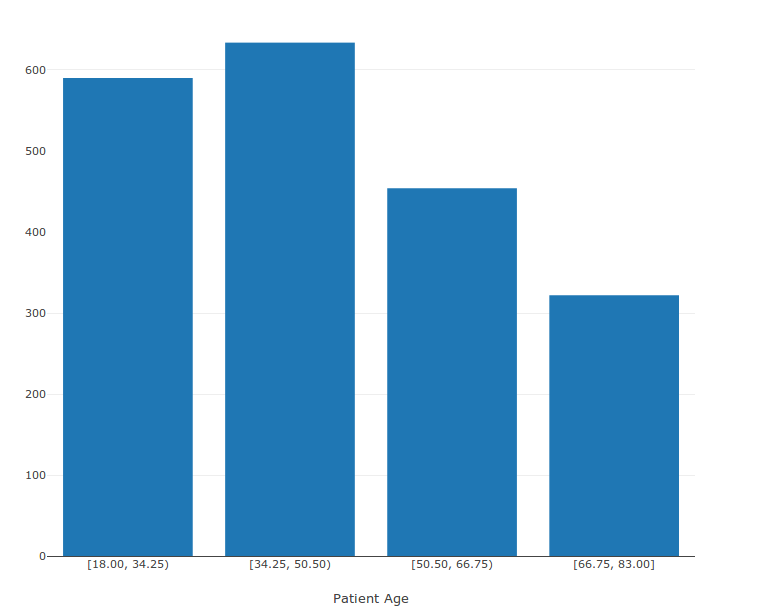
\includegraphics[width=\columnwidth]{figures/1d-simple-hist.png}
  \captionof{figure}{An one-dimensional histogram with $\beta = 4$}
  \label{f:simple-1d-hist}
\end{minipage}%
\begin{minipage}{.5\textwidth}
  \centering
  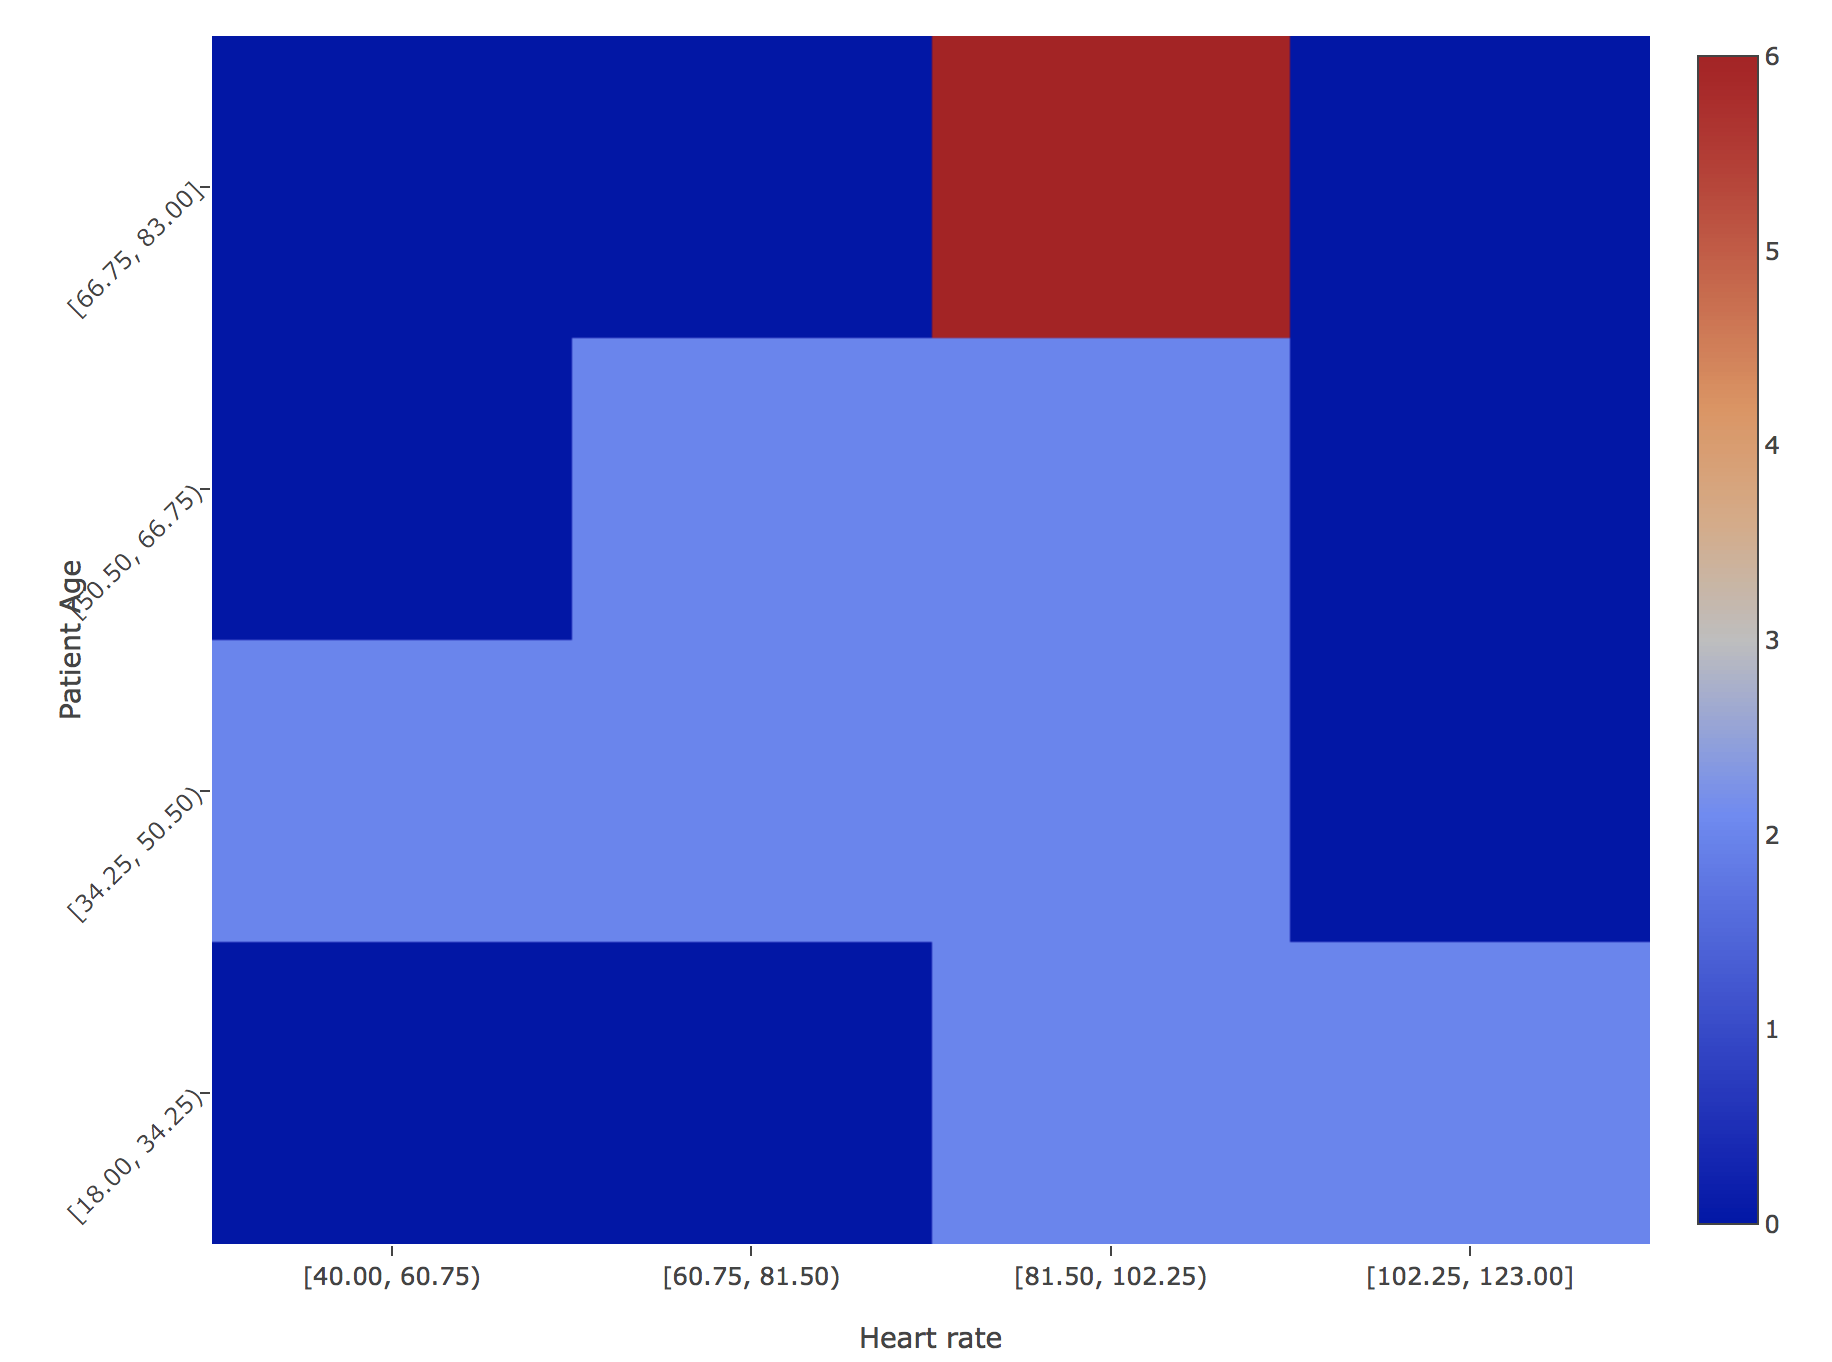
\includegraphics[width=\columnwidth]{figures/2d-simple-hist.png}
  \captionof{figure}{A two-dimensional histogram / heatmap with $\beta = 4$}
  \label{f:simple-2d-hist}
\end{minipage}
\end{figure}

\begin{figure}[t]
\centering
\begin{minipage}{.5\textwidth}
  \centering
  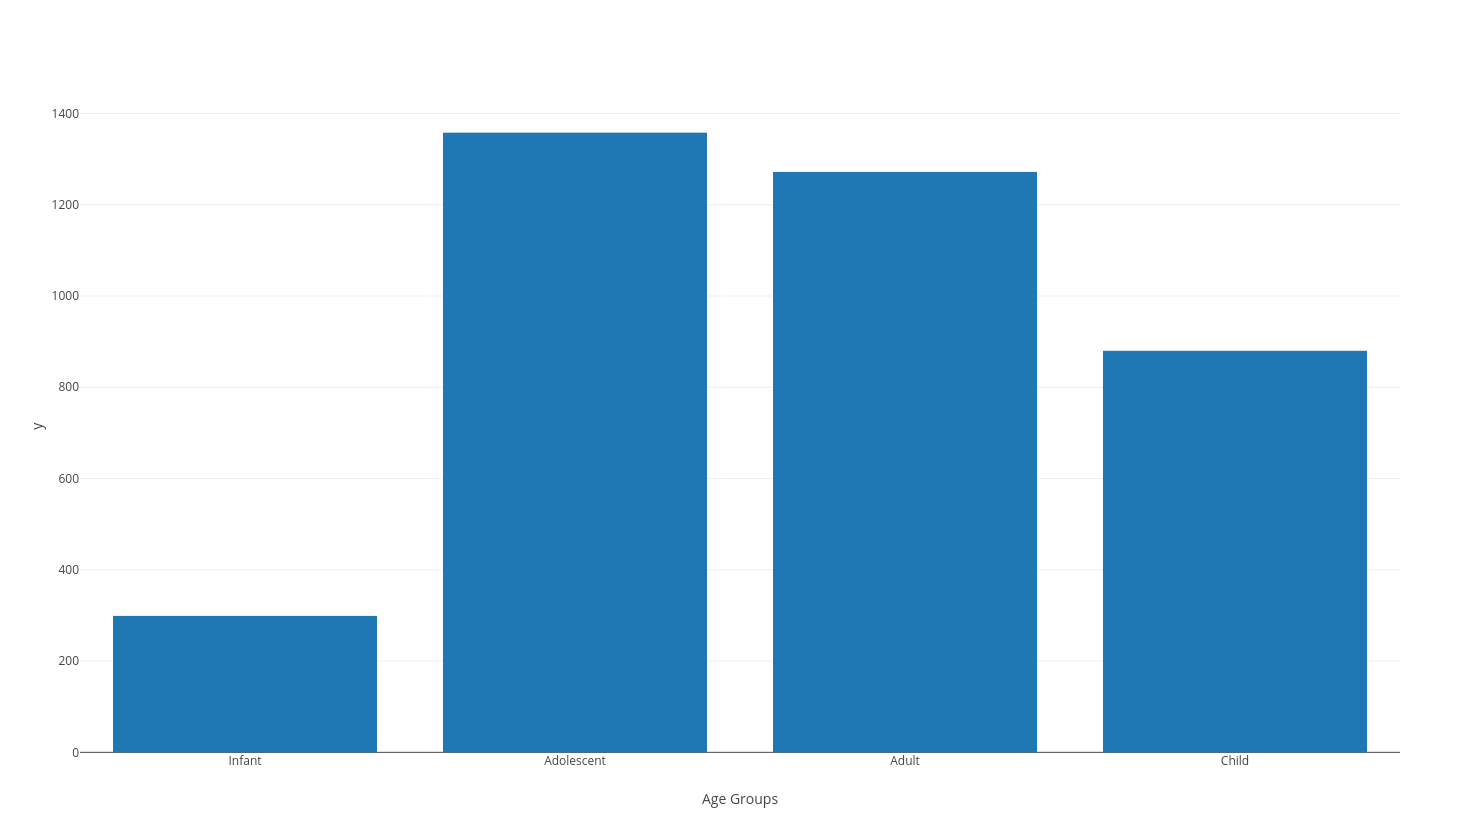
\includegraphics[width=\columnwidth]{figures/AgeGroups.png}
  \captionof{figure}{One-dimensional histogram displaying Age Groups}
  \label{f:simple-1d-categorical-hist}
\end{minipage}%
\begin{minipage}{.5\textwidth}
  \centering
  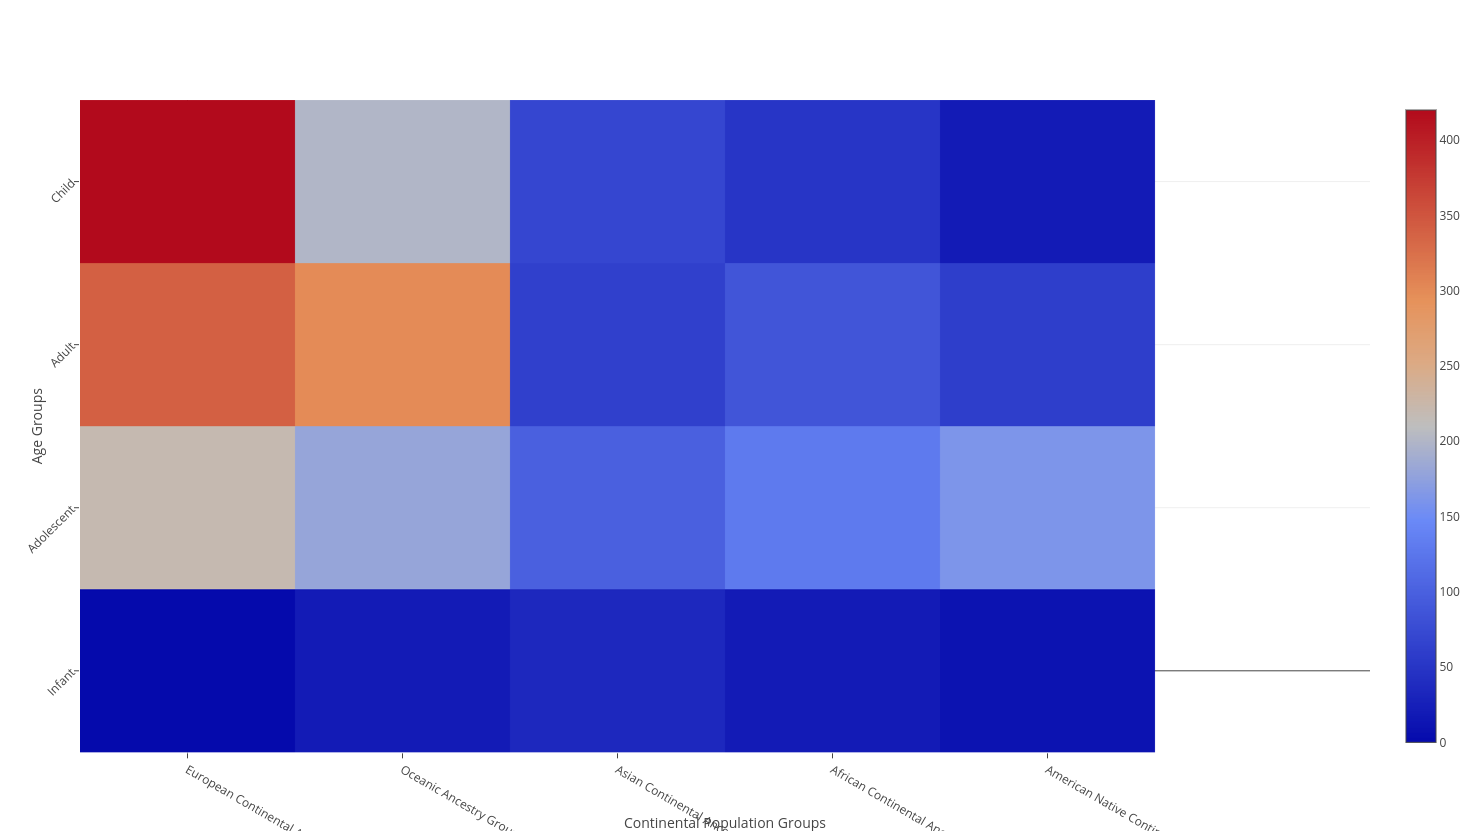
\includegraphics[width=\columnwidth]{figures/AgeGroups_PopulationGroups.png}
  \captionof{figure}{A two-dimensional histogram displaying Age Groups with Continental Population Groups}
  \label{f:simple-2d-categorical-hist}
\end{minipage}
\end{figure}


Similarly, in figures \ref{f:simple-1d-categorical-hist} and \ref{f:simple-2d-categorical-hist} we present two more histograms, but with categorical values.
The attribute ``Age Groups" in \ref{f:simple-1d-categorical-hist} is separated in four disjoint categories; ``Infant", ``Adolescent", ``Child" and ``Adult".
In \ref{f:simple-2d-categorical-hist} we present demographic information (attribute ``Continental Population Groups") in relation with ``Age Groups".





\subsection{Algorithms for Privacy Preserving Histograms}\label{ss:histogram-algos}
Histograms are one of the simplest ways to visualize and easily understand data; rendering them very useful in many data analysis applications.
As we already mentioned, histograms consist of bars that are mutually disjoint and their heights are proportional to the counts of values in the corresponding ranges.

\textbf{Challenges with Privacy-Preserving Histograms}: The textbook algorithm splits the dataset to buckets and consecutively for each item it increments the corresponding ``bucket-counter".
Implementing this algorithm with respect to the privacy of the dataset introduces the problem that for each value it is not trivial to find the bucket that this specific value should be placed.

For instance, let us suppose that we are constructing the histogram in figure \ref{f:simple-1d-categorical-hist}.
In this case $\beta = 4$, thus the algorithm should obliviously split the values into four disjoint buckets.
The range of each bucket is computed considering the $\beta$ parameter, as well as the minimum and maximum age in the dataset.
In this specific example, the minimum age is $18$, while the maximum is $83$.
Having $\beta = 4$ results to bucket-range $(83 - 18) / 4 = 16.25$.
Therefore, the ranges for attribute ``Patient Age" are formed as follows: $[18, 34.25),$ $[34.25, 50.50),$ $[50.50, 66.75),$ $[66.75, 83]$.
Consecutively, for each patient in the dataset the algorithm calculates the number of bucket that the patient belongs by dividing his/her value with the bucket-range; however, this index is encrypted.
Finally, the algorithm iterates through all $\beta$ buckets and obliviously adding $\enc{1}$ if the bucket is the correct one, or $\enc{0}$ otherwise.

The aforementioned algorithm works for numerical values; however, the one for categorical values is very similar.
Bucket-range is fixed to one, and $\beta$ equals to all different possible values in the dataset.
Also, there is no notion of terms minimum and maximum in categorical values.


\subsubsection{Privacy Preserving Histogram Computation: A Naive Approach}\label{sss:histogram-simple}
As we mentioned in section \ref{s:two-types-of-data}, we have separated our algorithms in two major categories, for categorical and for numerical data.
The procedure described in \ref{ss:histogram-algos} is shown in algorithms \ref{a:1d-simple-histogram-categorical} and \ref{a:1d-simple-histogram-numerical}.
These algorithms iterate through all $N$ items and check all possible cells for that item.
When the correct cell is found, they increment the corresponding counter.
The former is tailored to categorical datasets, while the latter is tailored to numerical/continuous values.

\import{./}{algorithms/hist_simple_categorical.tex}

\import{./}{algorithms/hist_simple_numerical.tex}

Both algorithms are straightforward and simple to understand, however, not very efficient.
In the following subsections we delve into details for the privacy preserving algorithms that are based in the same idea, but leverage \texttt{SIMD} operations.


\subsubsection{Privacy Preserving Histograms for Categorical Values}\label{sss:histogram-categorical}
\textbf{One-Dimensional Histograms}: In algorithm \ref{a:1d-histogram-categorical} we present the privacy preserving algorithm of an one-dimensional (1D) histogram for categorical values.
In simple words, categorical data means that the values are discrete.
Hence, the second parameter in the algorithm (dubbed $P$) is the number of possible choices that exist in $array[N]$.
The input data is given in the form of a private array/vector.

The algorithm creates a boolean array of equal size as the input data, and then for each possible encrypted value of the dataset checks (line 3) and counts (line 4) its occurrences.
Method {\fontfamily{lmss} $\textsc{Sum}$} is the same as in algorithm \ref{a:sum}.
Finally, the counts are gathered into a vector and returned -- still encrypted -- to the user.

\import{./}{algorithms/1d_hist_categorical.tex}



\textbf{Multi-Dimensional Histograms}: In algorithm \ref{a:multidim-histogram-categorical} we present the privacy preserving algorithm of multi-dimensional histograms for categorical values.
As in algorithm \ref{a:1d-histogram-categorical}, here, the third parameter ($Ps$) is the number of possible choices that exist in $array$.
However, since here the input data is a private array with multiple dimensions $array[N][M]$, the possible values should express the possible values for each dimension.
Thus, $Ps$ is an array of $A$ slots, where $A$ is the number of attributes.


The algorithm that computes a private multi-dimensional histogram is similar to the one regarding one-dimensional histograms but also addresses the issue of having a histogram of arbitrarily many dimensions.
In case we had a fixed (\textit{i.e.} known \textit{a-priori}) number of dimensions the simplest solution would be to use nested loops, as many as the histogram dimensions.
Since the number of dimensions is not known, we have to think of something else.
We represent the multi-dimensional histogram as a serialized version with an one-dimensional array (a vector) instead of using a multi-dimensional array (a matrix).
For example a 2-dimensional $3 \times 4$ histogram will be represented as a vector whose length is $ 12 $ ($= 3 \cdot 4$), and a $3 \times 4 \times 5$ 3-dimensional histogram wit a vector of length $ 60 $ ($= 3 \cdot 4 \cdot 5$)

When it comes to indexing if we wish to access the 2-dimensional $N \times M$ histogram represented as an one-dimensional at row $ i $ and column $ j $, instead of using $h[i][j]$ we use $h[i \cdot M + j]$.
Similarly, for the 3-dimensional $L \times N \times M$ histogram, $h[i][j][k]$ becomes $h[i \cdot N \cdot M + j \cdot M + k]$. So there needs to be a computation of a single index based on the multiple dimension indexes. In algorithm \ref{a:multidim-histogram-categorical}, the $positions$ vector holds this index for each record of the provided array, as can be seen in lines $ 6 $ and $ 7 $

Similarly to the 1D algorithm, the multi-dimensional one creates a boolean array ($eq$) for each possible histogram cell, which counts the occurrences of that cell in the $positions$ vector, as can be seen in lines $12$ and $13$ of algorithm \ref{a:multidim-histogram-categorical}.
\import{./}{algorithms/multdim_hist_categorical.tex}



\subsubsection{Privacy Preserving Histograms for Numerical Values}\label{sss:histogram-numerical}

\textbf{One-Dimensional Histograms}: In algorithm \ref{a:1d-histogram-numerical} we present the privacy preserving algorithm of one-dimensional (1D) histograms for numerical values.
In contrast with the categorical data, numerical data are not discrete, which means that the buckets in which the histogram will separate the dataset should be fixed (the $\beta$ parameter, as mentioned in section \ref{s:histograms})

First and foremost, the input data is given in the form of a private array/vector of $N$ positions.
The second parameter is open (since the final results will eventually disclose it), and is the number of buckets/cells that the algorithm will create, namely the $\beta$ factor.
The two last parameters are also encrypted and are the minimum and maximum values found in the dataset/array (first parameter of the algorithm).
Those two parameters are necessary in order to determine for each element in the array in which cell should be placed.

This algorithm is very similar and in accord with algorithm \ref{a:1d-histogram-categorical}, however does some extra steps.
In lines 2 and 3, it first determines the width for each cell and then creates an array of $N$ elements that each one indicates the bucket that the element in the corresponding position of $array$ should be placed.
Consecutively, the algorithm creates another boolean array of equal size as the input data, and then for each possible encrypted value of the $cellMap$ checks (line 5) and counts (line 6) its occurrences.
Finally, the counts are gathered into a vector and returned -- still encrypted -- to the user.
Line 5 of algorithm \ref{a:1d-histogram-numerical} is more complex than line 3 of algorithm \ref{a:1d-histogram-categorical}, since the former has to check some corner cases of data that belong to the last bucket.

\import{./}{algorithms/1d_hist_numerical.tex}



\textbf{Multi-Dimensional Histograms}:
Algorithm \ref{a:multidim-histogram-numerical} implements multi\hyp dimensional histograms for numerical, \textit{i.e.} continuous data.
The algorithm is a straightforward generalization of algorithm \ref{a:1d-histogram-numerical}.
Similarly, for each specified attribute we compute the corresponding cell width, that depends on the minimum and maximum values and the specified cell number of that attribute.
Consecutively, we compute the $positions$ vector containing the histogram cell for each one of the $N$ rows of $array$.
Like in algorithm \ref{a:multidim-histogram-categorical}, the $positions$ array contains single indexes that correspond to multiple indexes according to the procedure described above in section \ref{sss:histogram-categorical}.


\import{./}{algorithms/multdim_hist_numerical.tex}



\subsubsection{Filters in Privacy Preserving Histograms}\label{sss:histogram-filters}
Although histograms are one of the simplest ways to visualize and easily understand data, they also come with some limitations.
For instance, it is difficult to visualize in one image more than three different attributes.
Even though we can compute histograms of arbitrarily many dimensions, even a 3D representation can sometimes  be very obscure and difficult to understand.

Oftentimes, one needs to take into consideration multiple attributes in order to get meaningful results back.
However, adding more attributes to the computed histogram is not always an option as for the reasons described above, the output could be obscure or even useless whatsoever.

For all those reasons, we have implemented a \textit{filtering} technique in order to take more attributes into consideration for the secure computation.
With filtering, the user is able to select a histogram computation over some attributes, and also specify some extra constraints over the same or different attributes.
Each tuple from the dataset has to meet the specified criteria / filters in ordered to be counted in the resulting histogram.

The specified filters are represented as a list of constraints that should be met.
Each constraint is defined by the corresponding attribute, an operator ( one of $\{<, >, =\}$ for continuous attributes, and just $=$ for categorical ones) and a value.
Also a boolean operator (\textit{e.g.} \texttt{AND, OR, XOR}) that will be applied between the different constraints is specified.


For example, one could want to see the correlation of age and height but only for a subset of the dataset.
Let us suppose two examples, in the first we want the subset that include all patients of age above $45$, while in the second subset we want to include all patients of age above $45$ and that in the same time weigh less than $90$ kg.
This can be achieved with two requests of two\hyp dimensional histograms on the attributes \textit{Patient Age} and \textit{Height (cm)} that also includes the filters \textit{Patient Age} $ > 45$, and the second additionally have the limitation that \textit{Weight (kg)} $ < 90$, and also the boolean operator \texttt{AND} between them.
These will result to two 2\hyp dimensional histograms (heatmap) with axes the \textit{Patient Age} and \textit{Height (cm)} attributes, but at the same time the results will be restricted by the selection of these filters.
The described example from above, is depicted in figures \ref{f:2d_no_filter}, \ref{f:2d_1_filter} and \ref{f:2d_filter}, in which the impact of the filters is obvious.


\begin{figure}[t]
  \centering
  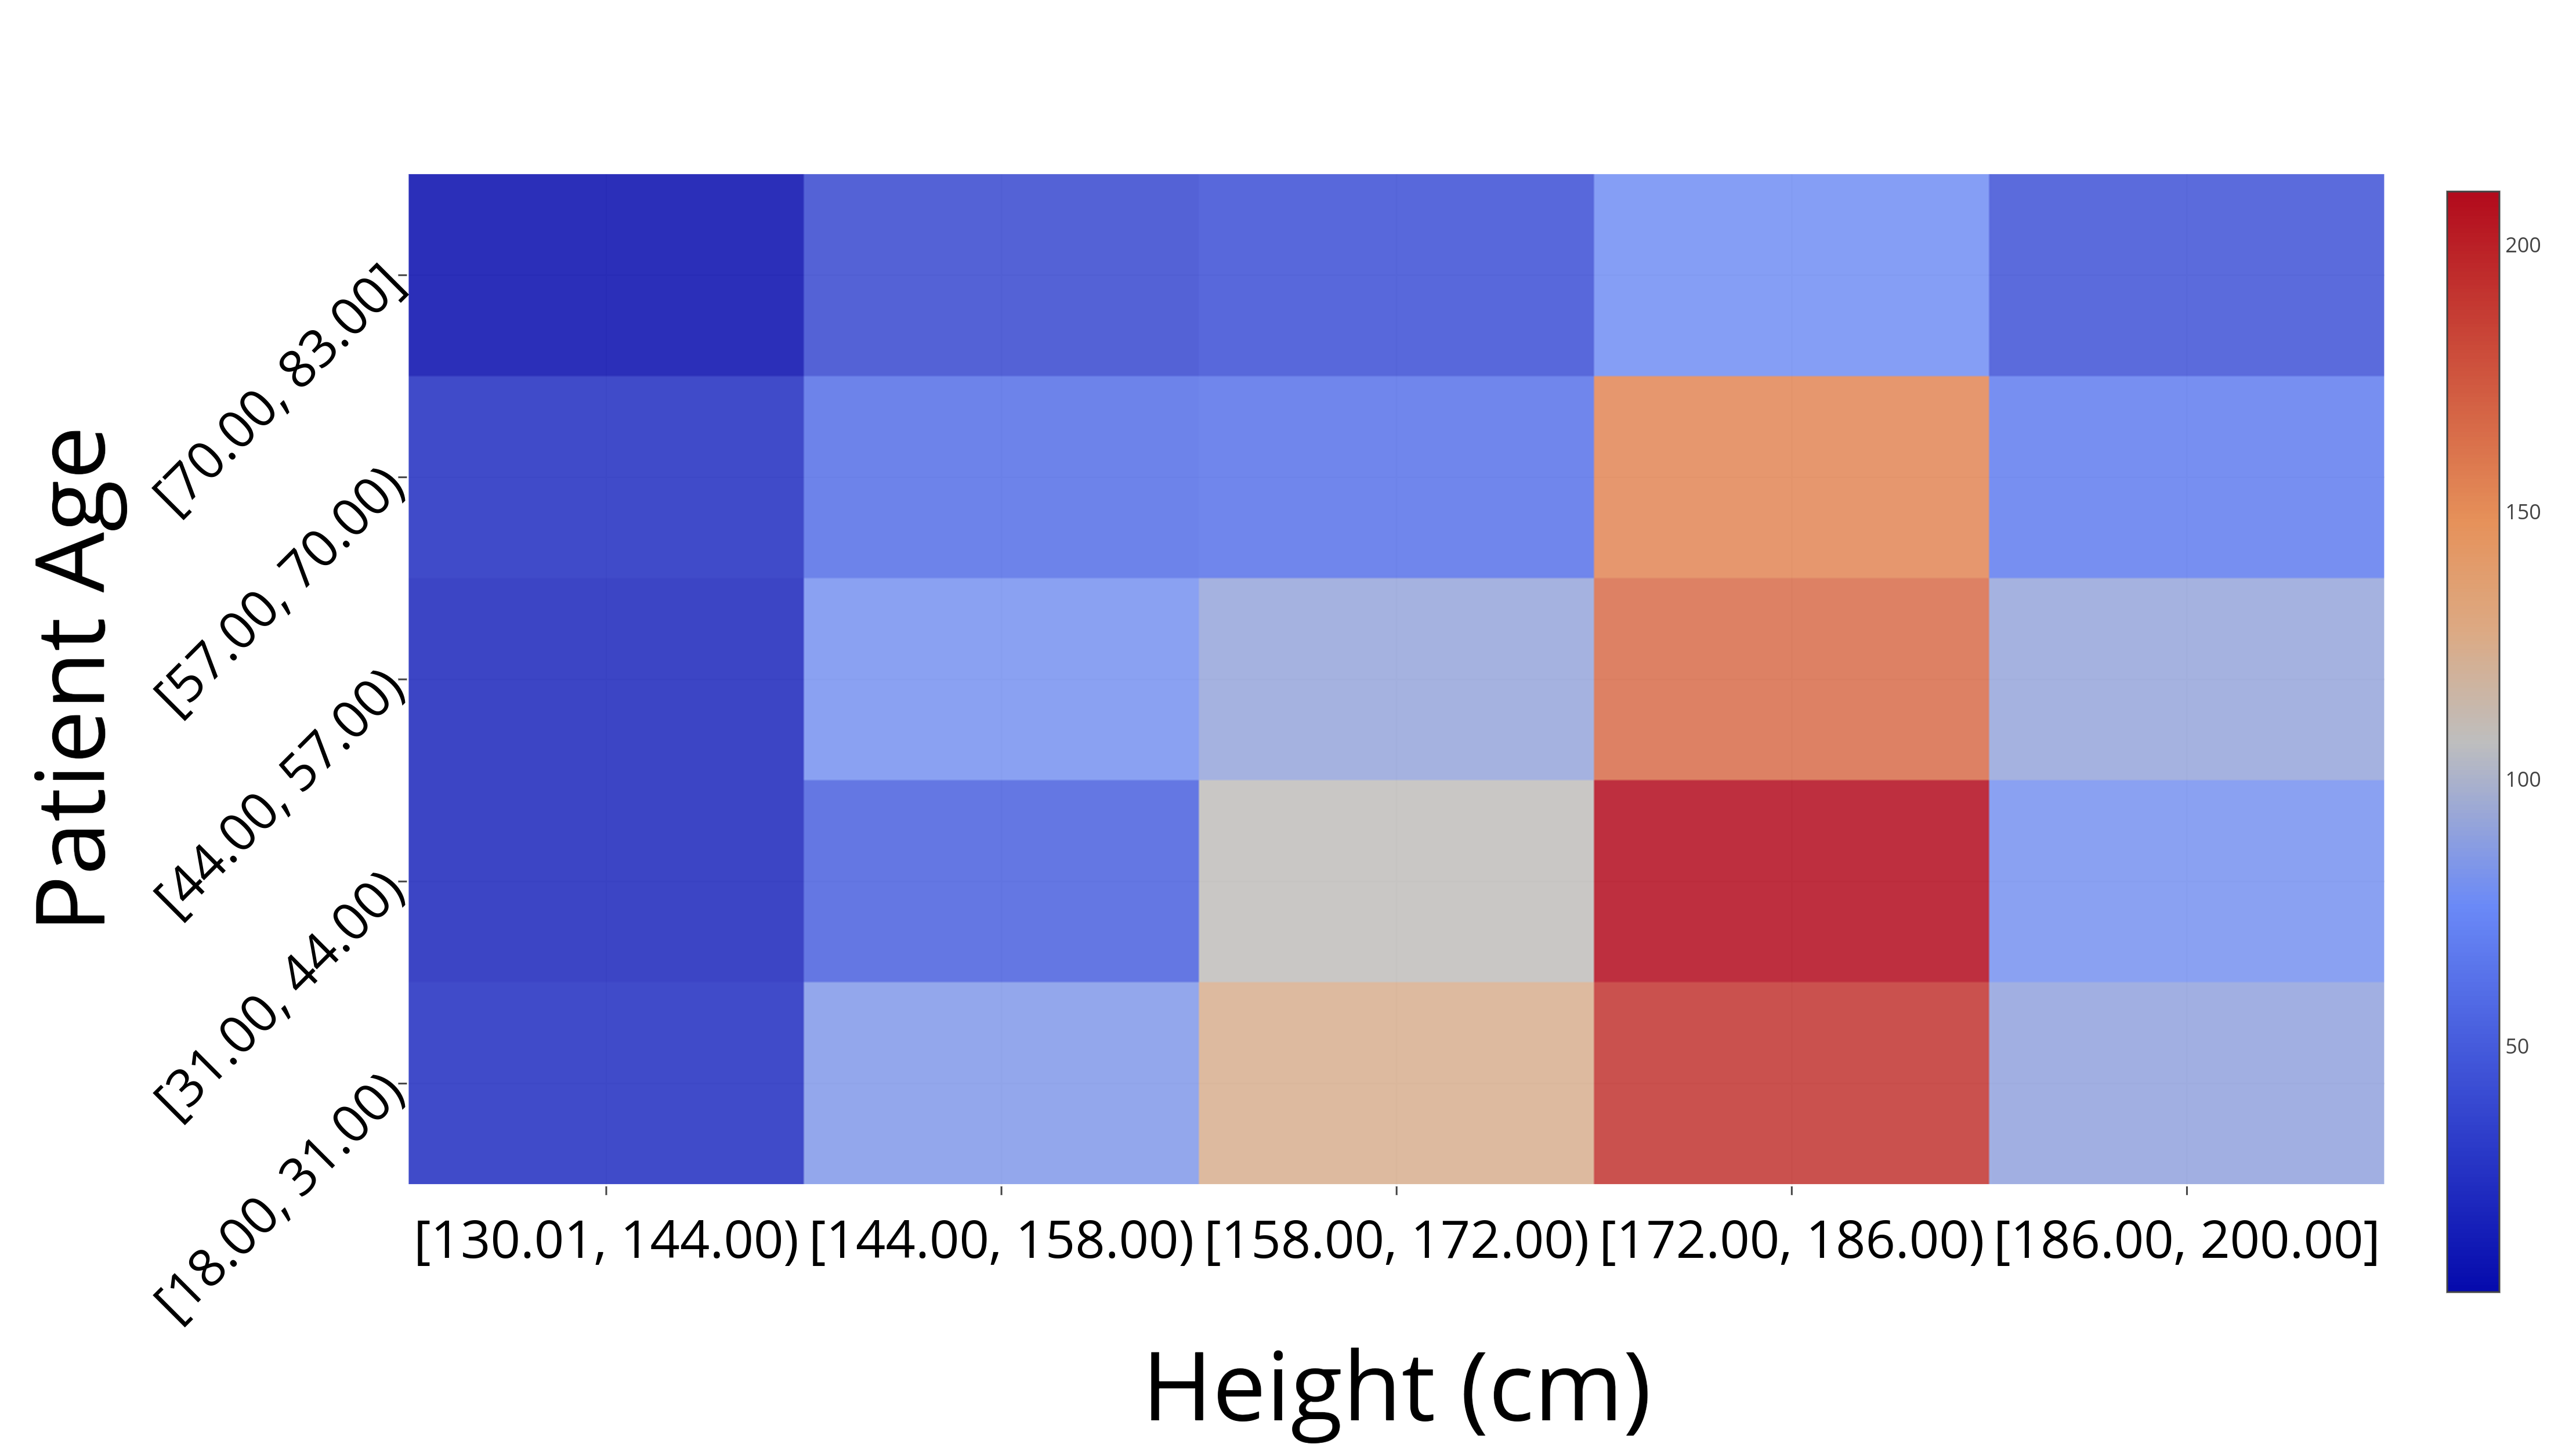
\includegraphics[width=0.8\linewidth]{figures/2d_no_filter.png}
  \caption{Histogram on \textit{Patient Age} and \textit{Height (cm)} with no filters}
  \label{f:2d_no_filter}
\end{figure}

\begin{figure}[th]
\centering
\begin{minipage}{.5\textwidth}
  \centering
  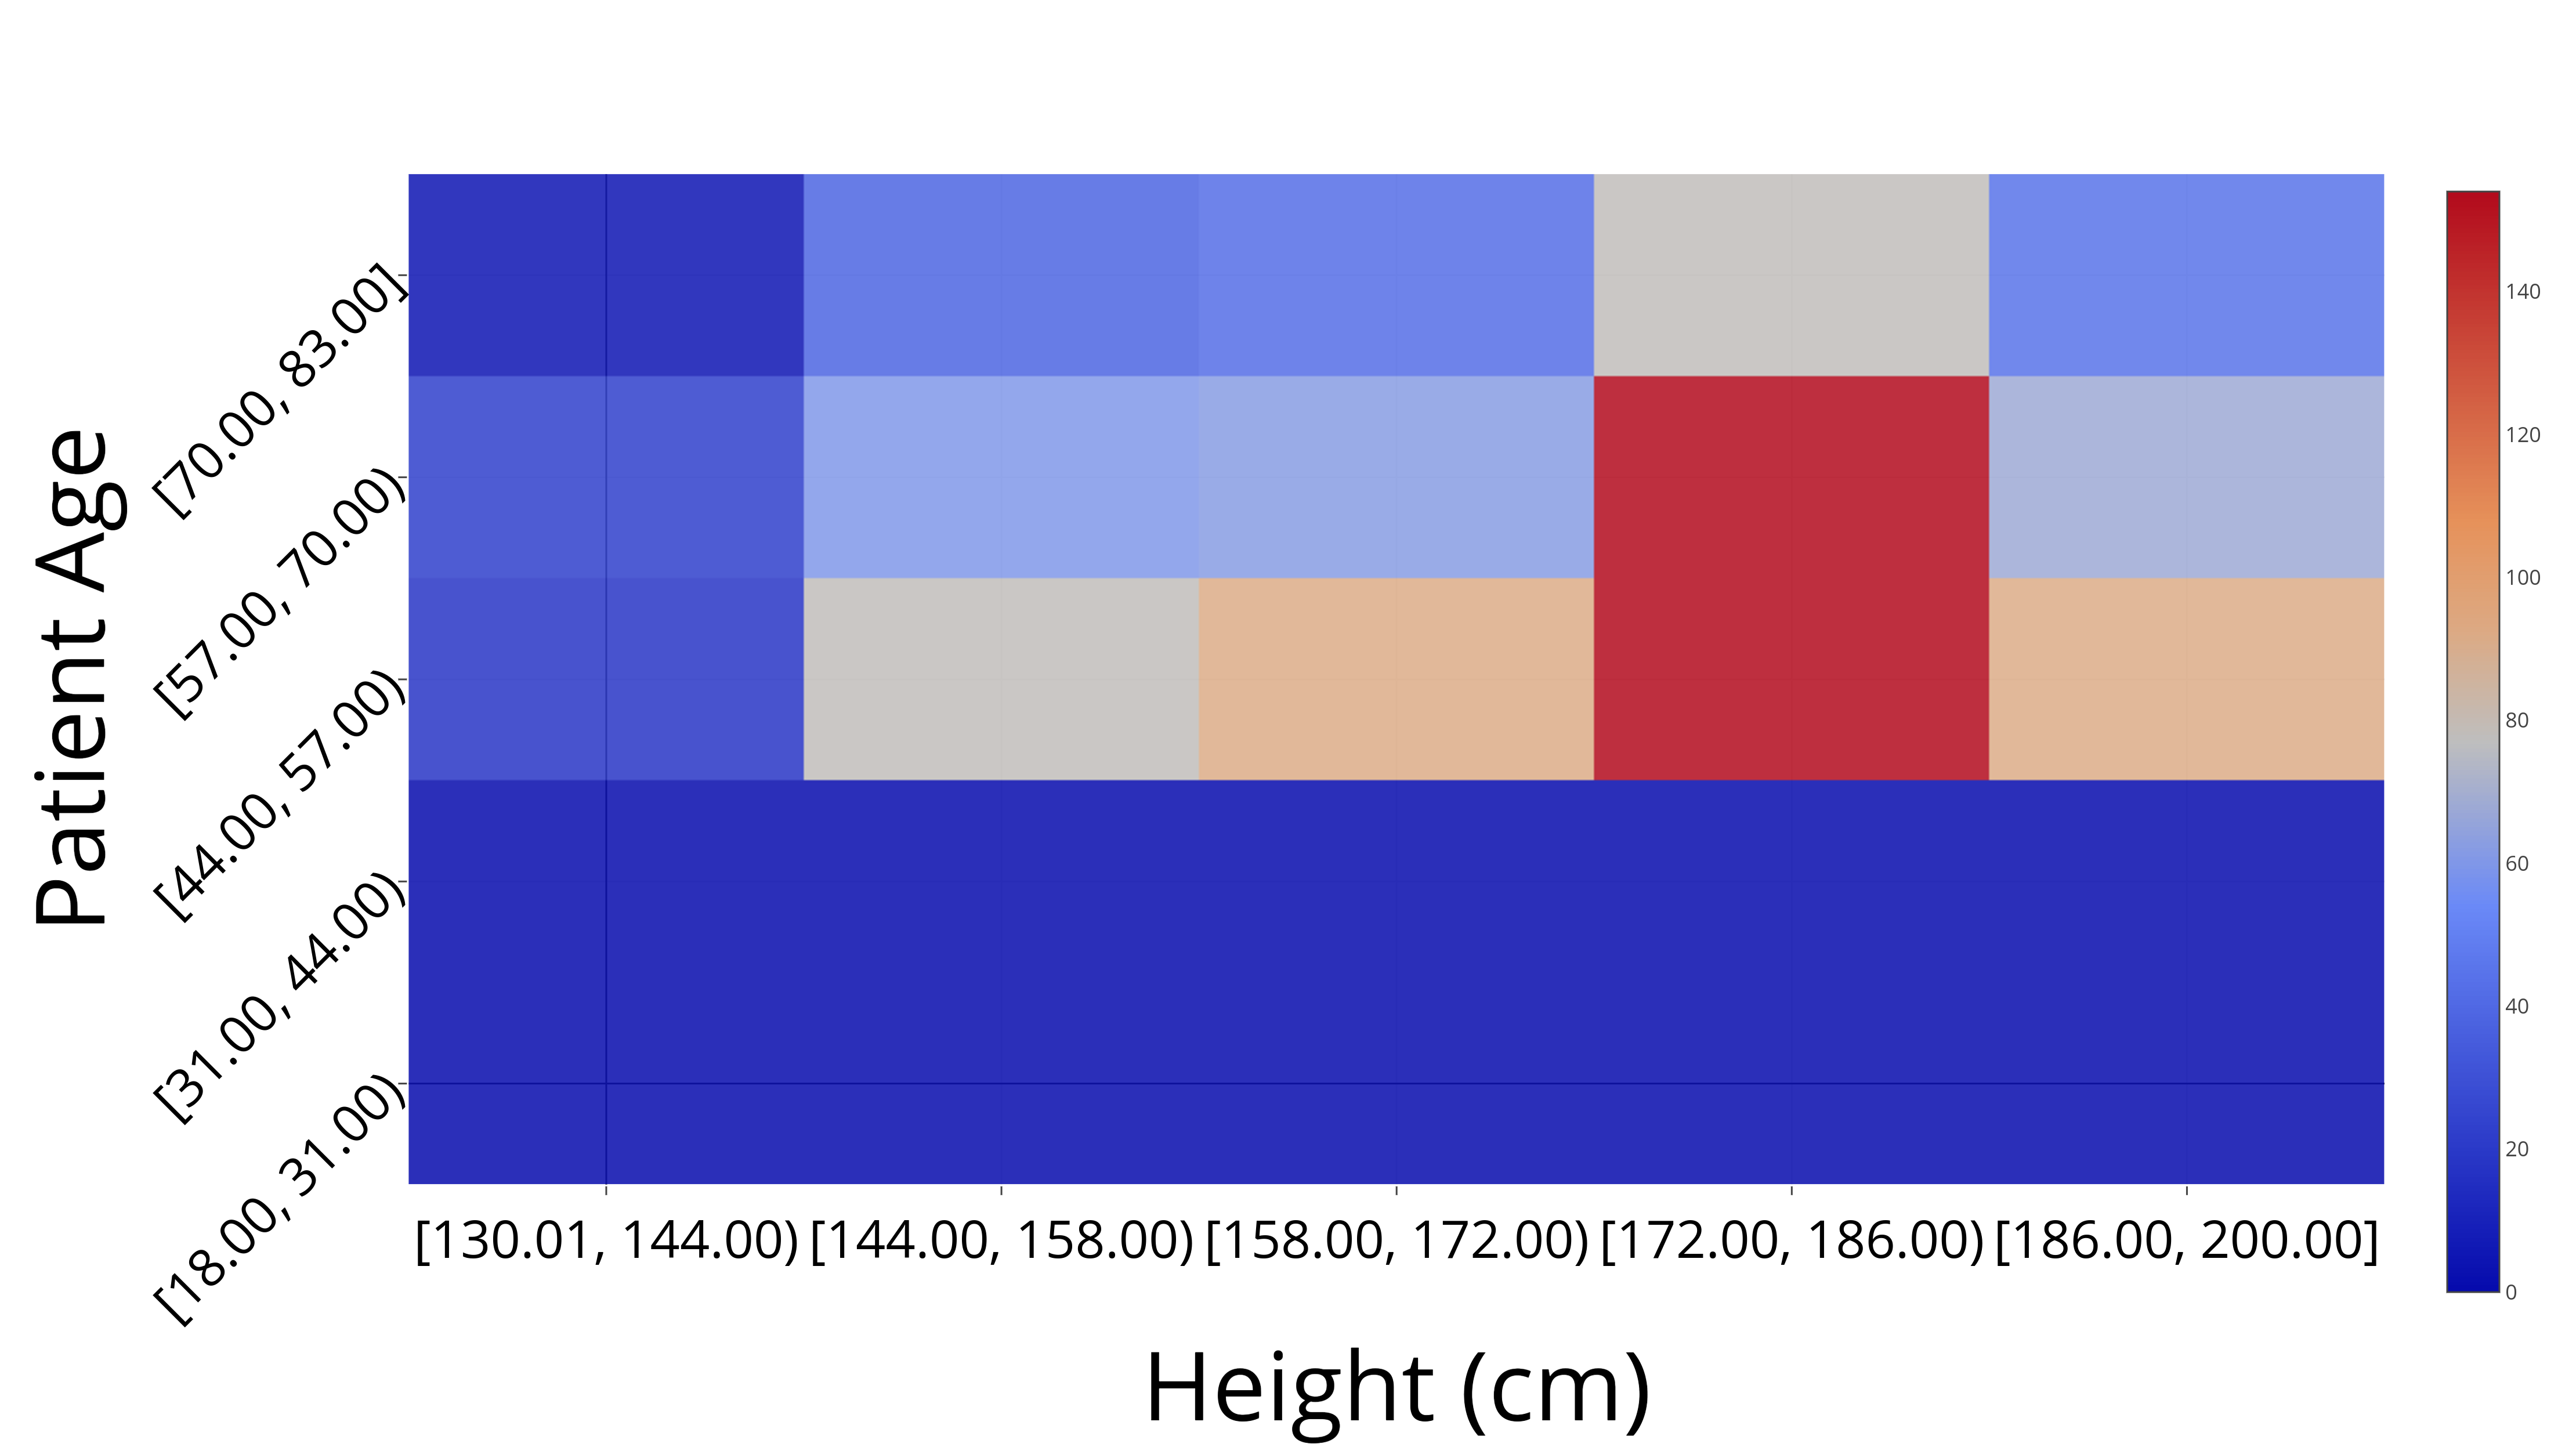
\includegraphics[width=\columnwidth]{figures/2d_1_filter.png}
  \captionof{figure}{Histogram on \textit{Patient Age} and \textit{Height (cm)} with filters on \textit{Patient Age}}
  \label{f:2d_1_filter}
\end{minipage}%
\begin{minipage}{.5\textwidth}
  \centering
  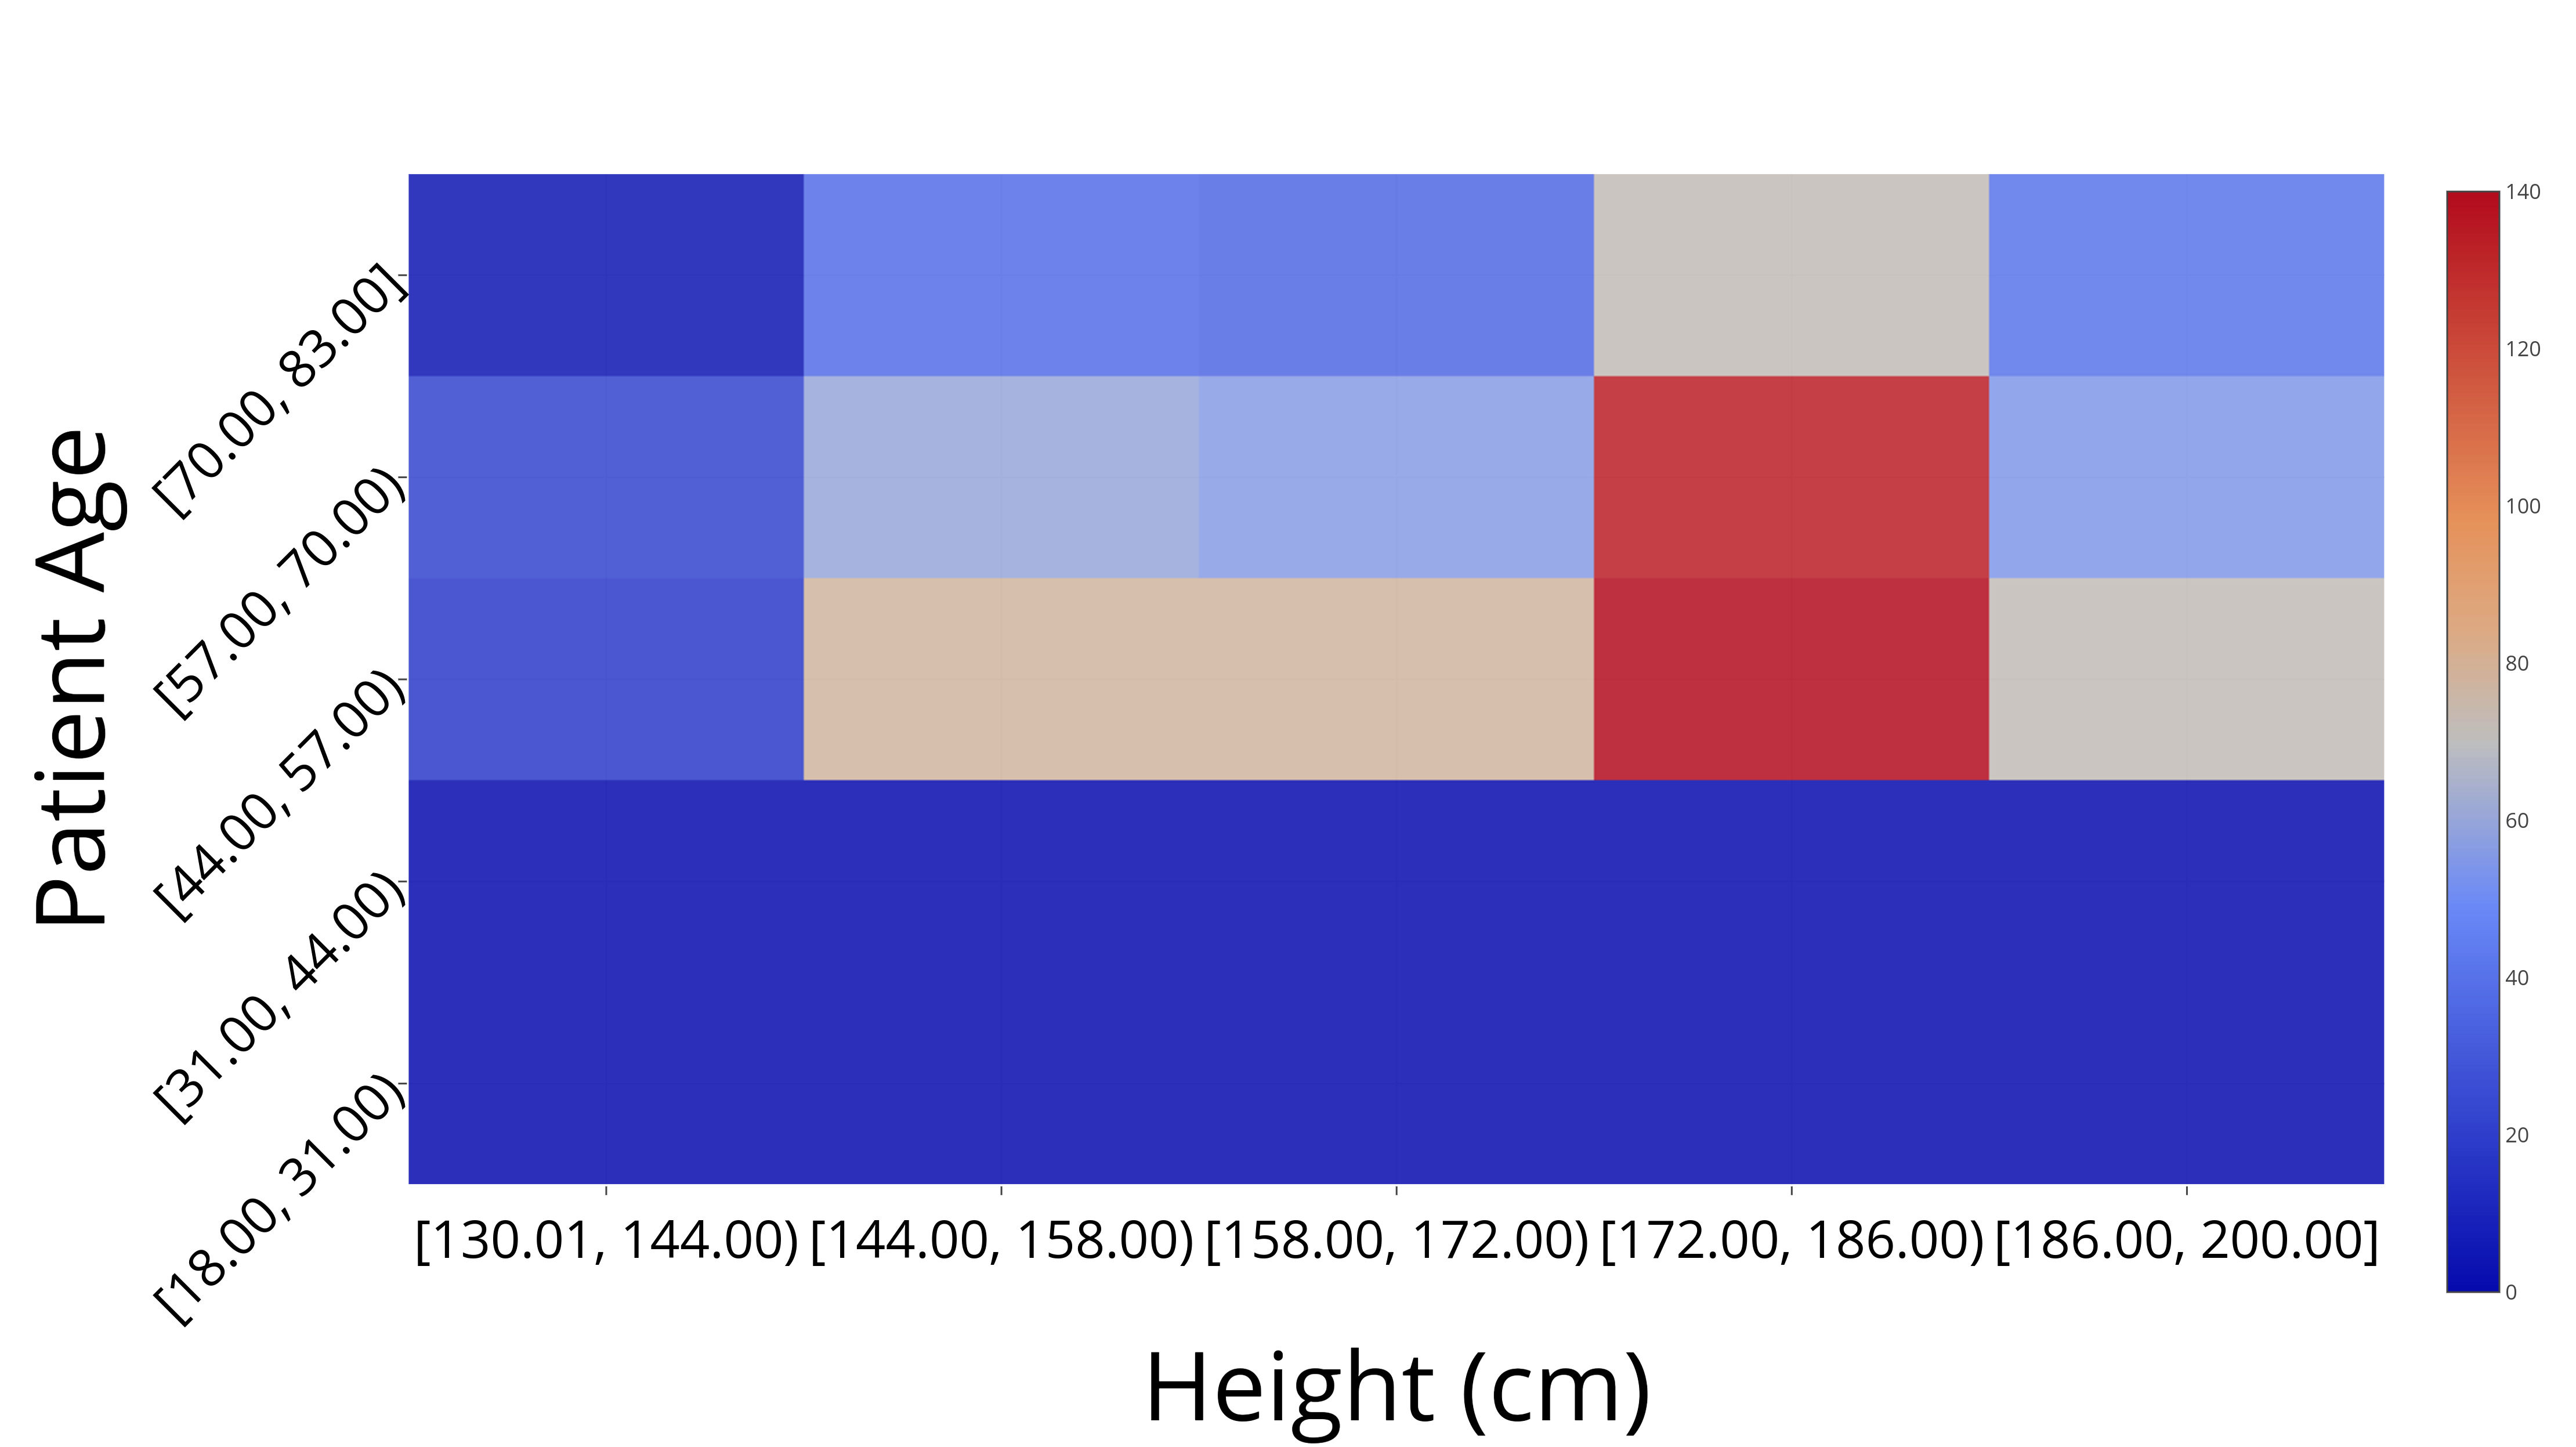
\includegraphics[width=\columnwidth]{figures/2d_filter.png}
  \captionof{figure}{Histogram on \textit{Patient Age} and \textit{Height (cm)} with filters on \textit{Patient Age} and \textit{Weight (kg)}}
  \label{f:2d_filter}
\end{minipage}
\end{figure}


Another example can be an one\hyp dimensional histogram on Body mass Index (BMI) on the subset of patients that weigh more than $90$ kg or are less than $170$ cm in height.
This can be achieved withl a request of an one\hyp dimensional histogram on the attribute \textit{BMI (kg/msq)} that also includes the filters \textit{Weight (kg)} $ > 90$, \textit{Height (cm)} $ < 170$, and also the boolean operator \texttt{OR} between them.
The effect of this example can be found in figures \ref{f:1d_no_filter} and \ref{f:1d_filter}.

\begin{figure}
\centering
\begin{minipage}{.5\textwidth}
  \centering
  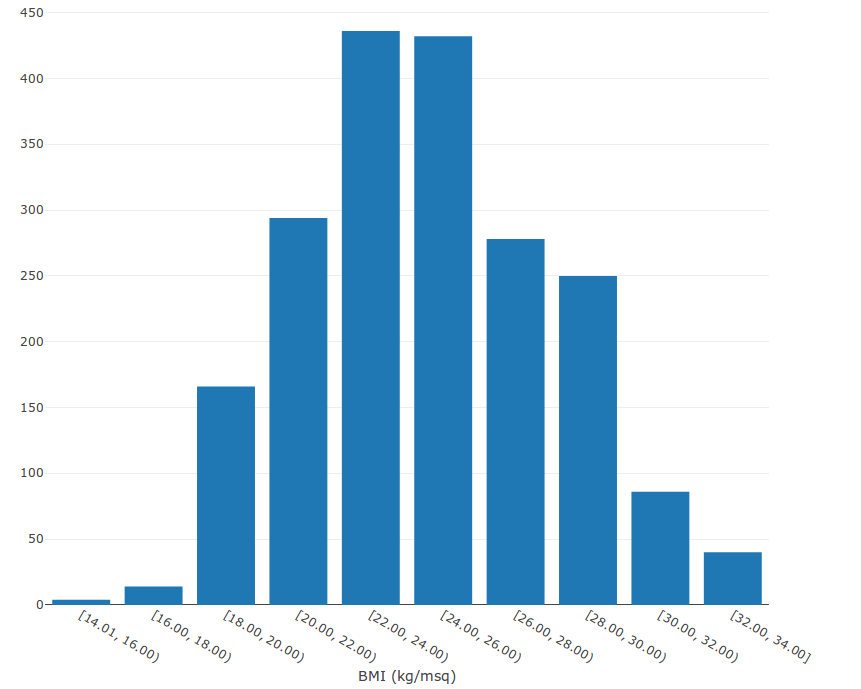
\includegraphics[width=\columnwidth]{figures/1d_no_filter.png}
  \captionof{figure}{Histogram on \textit{BMI (kg/msq)} with no filters}
  \label{f:1d_no_filter}
\end{minipage}%
\begin{minipage}{.5\textwidth}
  \centering
  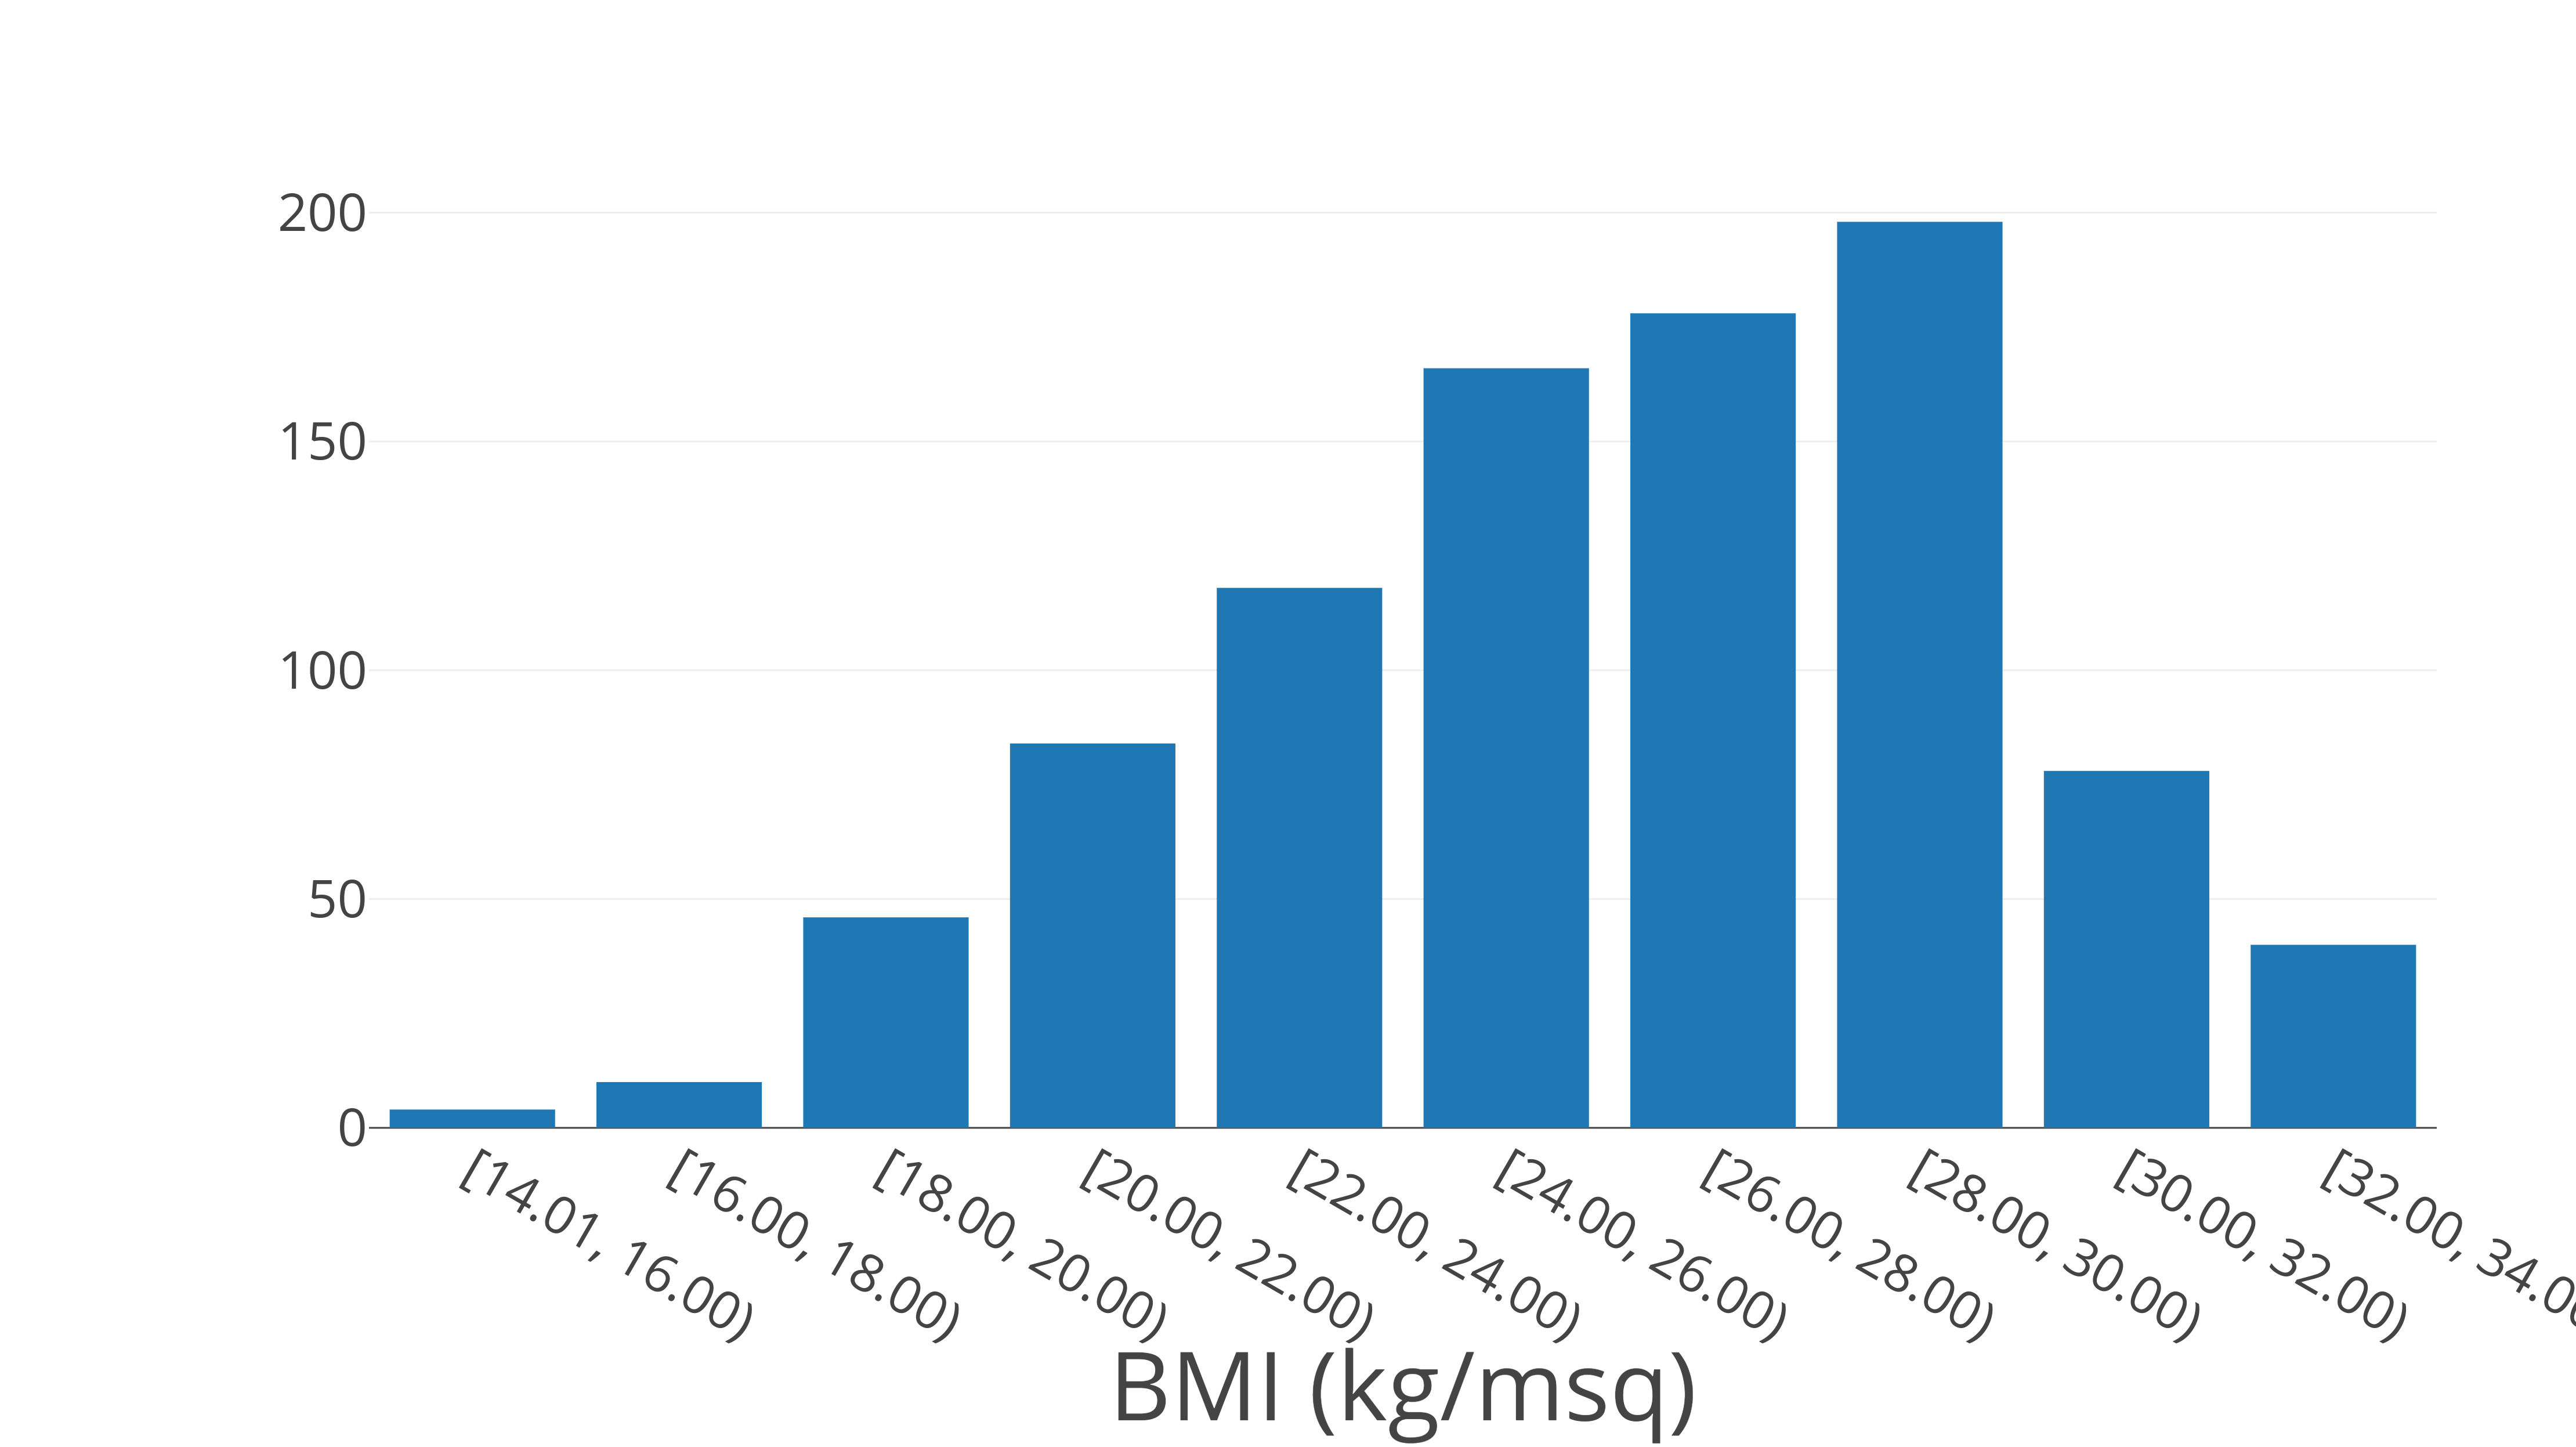
\includegraphics[width=\columnwidth]{figures/1d_filter.png}
  \captionof{figure}{Histogram on \textit{BMI (kg/msq)} with filters on \textit{Height (cm)} and \textit{Weight (kg)}}
  \label{f:1d_filter}
\end{minipage}
\end{figure}

\import{./}{algorithms/filters.tex}

The way that \textit{filters} have been implemented is by constructing a vector of size $N$ (\textit{i.e.} as long as the number of tuples in the dataset), that works as a boolean mask corresponding to the specified constraints.
Each position of that vector corresponds to a data tuple from the dataset.
If that tuple satisfies all the specified constraints, then the vector should have the (encrypted) value \texttt{True} in that position, or (encrypted) \texttt{False} otherwise.
This vector then is taken into consideration when we build the histogram.
Only tuples which have ``scored'' \texttt{True} are counted into the histogram.

In algorithm \ref{a:filters-constraint-mask} the aforementioned vector is $constraintMask$.
In lines 14-20 we build this boolean mask for each constraint into the $eq$ vector, and in lines 21-27 we combine these vectors to build the total one, according to the specified boolean operator applied between them.

As you can see in algorithm \ref{a:filters-2d-histogram} which computes a multi\hyp dimensional histogram of categorical attributes, the application of this constraints is as simple as a private multiplication with the $N$-size vector $constraintMask$.
This SIMD operator can be seen in line 13.
Beyond this addition, the algorithm is identical to the standard multi\hyp dimensional histogram of categorical attributes as in algorithm \ref{a:multidim-histogram-categorical}.

\import{./}{algorithms/filters2.tex}





\section{Privacy Preserving ID3}\label{s:id3}

\fixme{many things from \href{http://www.pinkas.net/PAPERS/id3-final.pdf}{http://www.pinkas.net/PAPERS/id3-final.pdf}}

\import{./}{algorithms/id3_textbook.tex}


\begin{equation}\label{eq:entropy}
  H_C(T) = \sum_{i=1}^{l} - \frac{\mid T(c_i) \mid}{\mid T \mid} log{\frac{\mid T(c_i) \mid}{\mid T \mid}}
\end{equation}

\begin{equation}\label{eq:TgivenA}
  H_C(T \mid A) = \sum_{j=1}^{m} - \frac{\mid T(a_j) \mid}{\mid T \mid} H_C(T(a_j))
\end{equation}

\begin{equation}\label{eq:gain}
  Gain(A) = H_C(T) - H_C(T \mid A)
\end{equation}

\import{./}{algorithms/id3_pp.tex}


